\documentclass[unicode,11pt,a4paper,oneside,numbers=endperiod,openany]{scrartcl}

\usepackage{xcolor}
\usepackage{listings}
\usepackage{amsmath}

% Define custom verbatim environment with gray background
\lstnewenvironment{grayverbatim}{%
  \lstset{backgroundcolor=\color{gray!10}, % Adjust the shade of gray as desired
          frame=single,
          framerule=0pt,
          basicstyle=\ttfamily,
          breaklines=true,
          columns=fullflexible}
}{}

\lstnewenvironment{cppverbatim}{%
  \lstset{language=C++, % Set the language to C++
          backgroundcolor=\color{gray!10}, % Adjust the shade of gray as desired
          frame=single,
          framerule=0pt,
          basicstyle=\ttfamily,
          keywordstyle=\color{blue}, % Set the color for keywords
          commentstyle=\color{green!50!black}, % Set the color for comments
          stringstyle=\color{red}, % Set the color for strings
          breaklines=true,
          showstringspaces=false, % Don't show spaces within strings
          columns=fullflexible}
}{}

\usepackage{ifthen}
\usepackage[utf8]{inputenc}
\usepackage{graphics}
\usepackage{graphicx}
\usepackage{hyperref}

\pagestyle{plain}
\voffset -5mm
\oddsidemargin  0mm
\evensidemargin -11mm
\marginparwidth 2cm
\marginparsep 0pt
\topmargin 0mm
\headheight 0pt
\headsep 0pt
\topskip 0pt        
\textheight 255mm
\textwidth 165mm

\newcommand{\duedate} {}
\newcommand{\setduedate}[1]{%
\renewcommand\duedate {Due date:~ #1}}
\newcommand\isassignment {false}
\newcommand{\setassignment}{\renewcommand\isassignment {true}}
\newcommand{\ifassignment}[1]{\ifthenelse{\boolean{\isassignment}}{#1}{}}
\newcommand{\ifnotassignment}[1]{\ifthenelse{\boolean{\isassignment}}{}{#1}}

\newcommand{\assignmentpolicy}{
\begin{table}[h]
\begin{center}
\scalebox{0.8} {%
\begin{tabular}{|p{0.02cm}p{16cm}|}
\hline
&\\
\multicolumn{2}{|c|}{\Large\textbf{HPC Lab for CSE 2024 ---  Submission Instructions}}\\
\multicolumn{2}{|c|}{\large\textbf{(Please, notice that following instructions are mandatory: }}\\
\multicolumn{2}{|c|}{\large\textbf{submissions that don't comply with, won't be considered)}}\\
&\\
\textbullet & Assignments must be submitted to \href{https://moodle-app2.let.ethz.ch/course/view.php?id=22516}{Moodle} (i.e. in electronic format).\\
\textbullet & Provide both executable package and sources (e.g. C/C++ files, Matlab). 
If you are using libraries, please add them in the file. Sources must be organized in directories called:\\
\multicolumn{2}{|c|}{\textit{Project\_number\_lastname\_firstname}}\\
& and  the  file must be called:\\
\multicolumn{2}{|c|}{\textit{project\_number\_lastname\_firstname.zip}}\\
\multicolumn{2}{|c|}{\textit{project\_number\_lastname\_firstname.pdf}}\\
\textbullet &  The TAs will grade your project by reviewing your project write-up, and looking at the implementation 
                 you attempted, and benchmarking your code's performance.\\

\textbullet & You are allowed to discuss all questions with anyone you like; however: (i) your submission must list anyone you discussed problems with and (ii) you must write up your submission independently.\\
\hline
\end{tabular}
}
\end{center}
\end{table}
}
\newcommand{\punkte}[1]{\hspace{1ex}\emph{\mdseries\hfill(#1~\ifcase#1{Points}\or{Points}\else{Points}\fi)}}


\newcommand\serieheader[6]{
\thispagestyle{empty}%
\begin{flushleft}

\includegraphics[width=0.4\textwidth]{ETHlogo_13}
\end{flushleft}
  \noindent%
  {\large\ignorespaces{\textbf{#1}}\hspace{\fill}\ignorespaces{ \textbf{#2}}}\\ \\%
  {\large\ignorespaces #3 \hspace{\fill}\ignorespaces #4}\\
  \noindent%
  \bigskip
  \hrule\par\bigskip\noindent%
  \bigskip {\ignorespaces {\Large{\textbf{#5}}}
  \hspace{\fill}\ignorespaces \large \ifthenelse{\boolean{\isassignment}}{\duedate}{#6}}
  \hrule\par\bigskip\noindent%  \linebreak
 }

\makeatletter
\def\enumerateMod{\ifnum \@enumdepth >3 \@toodeep\else
      \advance\@enumdepth \@ne
      \edef\@enumctr{enum\romannumeral\the\@enumdepth}\list
      {\csname label\@enumctr\endcsname}{\usecounter
        {\@enumctr}%%%? the following differs from "enumerate"
	\topsep0pt%
	\partopsep0pt%
	\itemsep0pt%
	\def\makelabel##1{\hss\llap{##1}}}\fi}
\let\endenumerateMod =\endlist
\makeatother




\usepackage{textcomp}






\begin{document}


\setassignment
\setduedate{Monday 15 April 2024, 23:59 (midnight)}

\serieheader{High-Performance Computing Lab for CSE}{2024}
            {Student: CARLA JUDITH LOPEZ ZURITA}
            {Discussed with: RITVIK RANJAN}{Solution for Project 3}{}
\newline

\assignmentpolicy

In this report, we are solving Fisher's equation using the finite difference
method. The equation is given by:
\begin{align}
    \frac{\partial s}{\partial t} = D \nabla^2 u + R s (1 - s)
\end{align}
where $s$ is the concentration of a species, $D$ is the diffusion coefficient,
and $R$ is the reaction rate. The equation is solved on a 2D grid with
Dirichlet boundary conditions,
\begin{align}
    s(x, y, t) = 0.1 \quad \text{for} \quad x = 0, x = 1, y = 0, y = 1
\end{align}
and initial conditions is a circle of radius $1/8$ at the lower left quadrant the domain.
\section{Task: Implementing the linear algebra functions and the stencil
         operators [40 Points]}

The first part of the project consists in implementing the linear algebra functions and
the stencil operators. The linear algebra functions are implemented in the
\texttt{linalg.cpp} file. I implemented all the functions using
simple loops.
%  I tried using iterators but since the Fields class is a custom
% class, I decided to put that idea on hold until I have a better understanding of
% the code. 
Similarly, the stencil operators were implemented in the
\texttt{operators.cpp} file. Writing the interior grid points was very simple since
we already had the implementations for the boundary conditions.

Afterwards, I ran the code following the indications on the project description
and I got the following results in the terminal
\begin{grayverbatim}
================================================================================
                      Welcome to mini-stencil!
version   :: C++ Serial
mesh      :: 128 * 128 dx = 0.00787402
time      :: 100 time steps from 0 .. 0.005
iteration :: CG 300, Newton 50, tolerance 1e-06
================================================================================
--------------------------------------------------------------------------------
simulation took 0.203392 seconds
1513 conjugate gradient iterations, at rate of 7438.82 iters/second
300 newton iterations
--------------------------------------------------------------------------------
### 1, 128, 100, 1513, 300, 0.203392 ###
Goodbye!
\end{grayverbatim}
Which are the matching with the expected results.
Additionally, I got the following content for the \texttt{output.bin} file,
\begin{grayverbatim}
TIME: 0.005
DATA_FILE: output.bin
DATA_SIZE: 128 128 1
DATA_FORMAT: DOUBLE
VARIABLE: phi
DATA_ENDIAN: LITTLE
CENTERING: nodal
BRICK_ORIGIN: 0. 0. 0.
BRICK_SIZE: 1 1  1.0
\end{grayverbatim}
When plotting the results, they seem to be as expected; the population concentration is higher at
the lower left quadrant of the domain, which is matching with the initial condition.
\begin{figure}[!h]
    \centering
    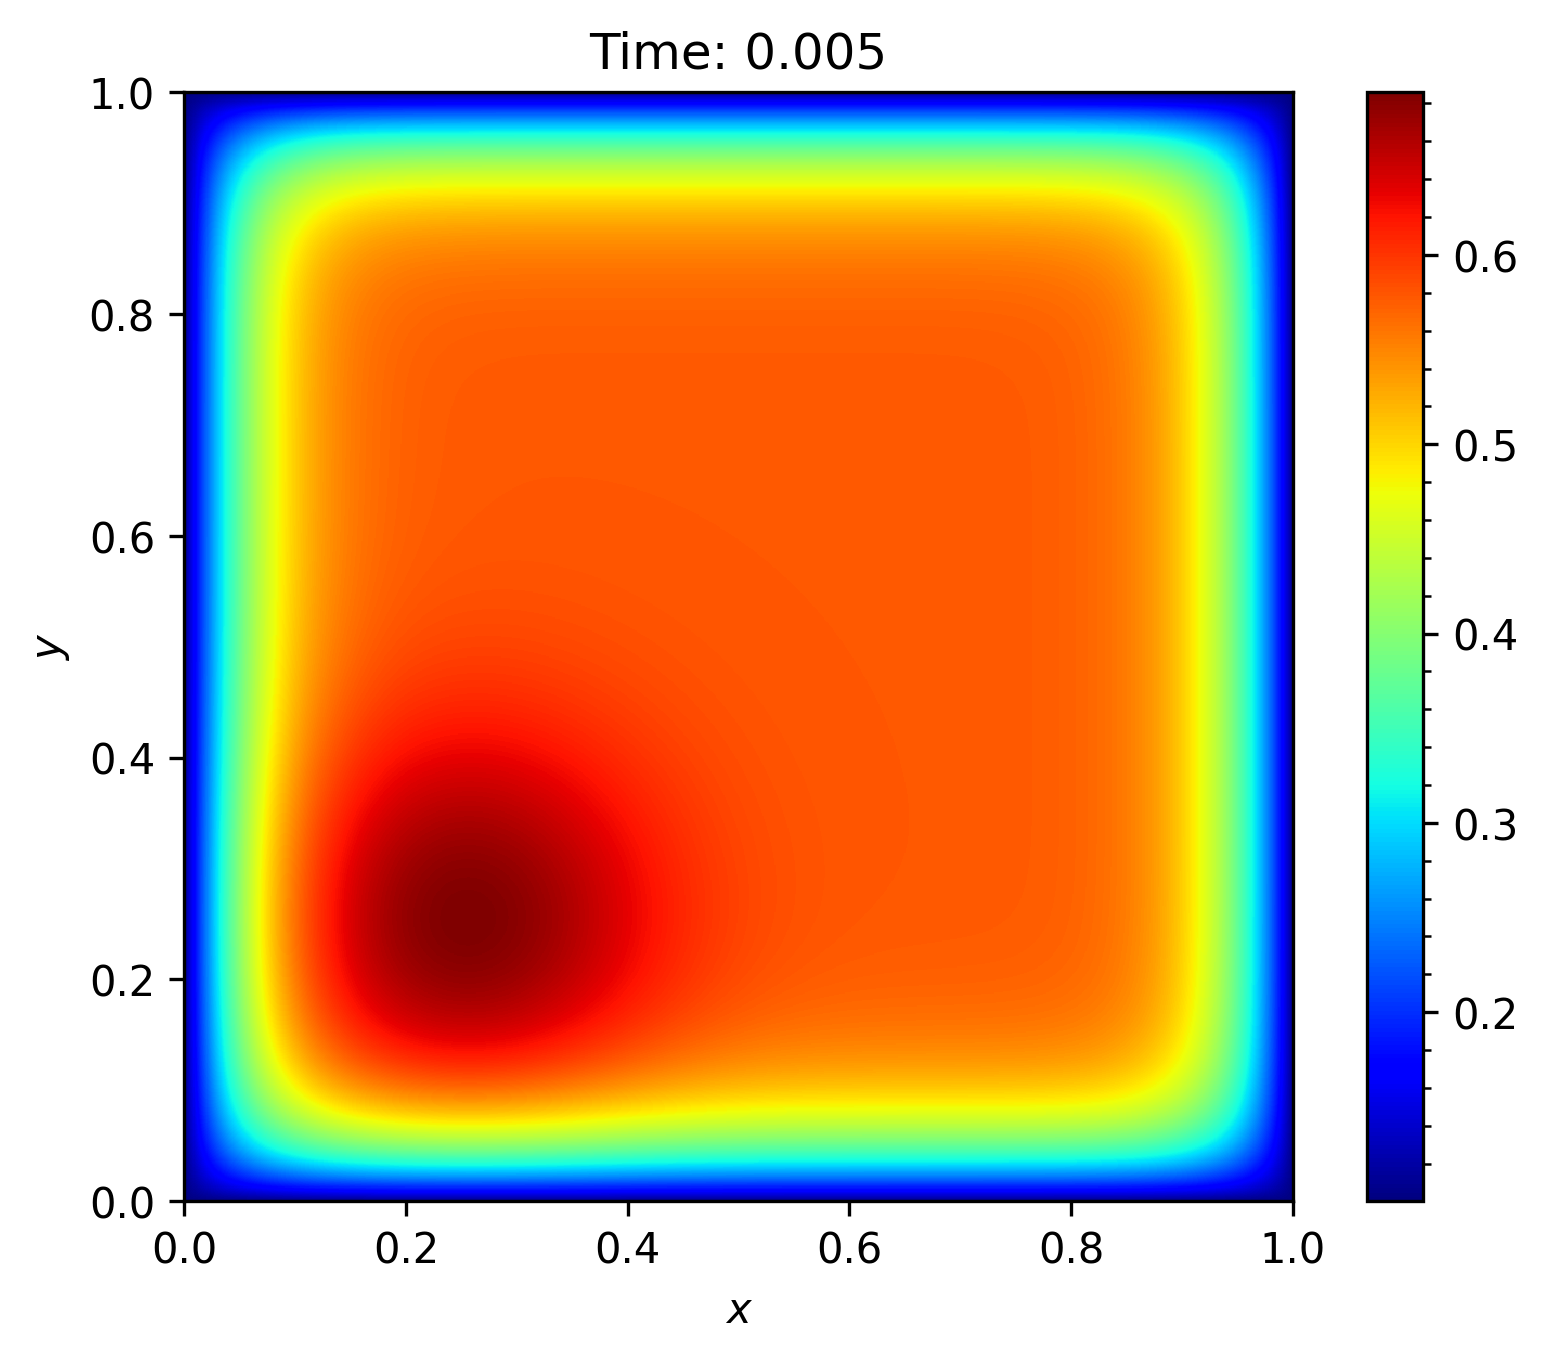
\includegraphics[width=0.5\textwidth]{../mini_app/output_high_res.png}
    \caption{The population concentration at time t = 0.005.}
    \label{im:final_time}
\end{figure}
Fig. \ref{im:final_time} shows the results corresponding to a run with a $1024 \times 1024$ grid.

\section{Task:  Adding OpenMP to the nonlinear PDE mini-app [60 Points]}
This section is dedicated to parallelizing the code using OpenMP and analyzing
the performance of the code, as well as some discussion regarding the results
and differences between the serial and parallel versions.

\subsection*{Welcome message and serial compilation}
We want to have different welcome messages for the serial and parallel versions.
This was done using the macro \texttt{\_OPENMP} which is defined when OpenMP is
enabled. The code is shown below.
\begin{cppverbatim}
#ifdef _OPENMP
#include "omp.h" // This line won't add the library if you don't compile with -fopenmp option.
#endif

...

#ifdef _OPENMP
    std::cout << "version   :: C++ OpenMP" << std::endl;
#pragma omp parallel
    {
        threads = omp_get_num_threads();
    }
    std::cout << "threads   :: " << threads << std::endl;
#else
    std::cout << "version   :: C++ Serial" << std::endl;
#endif
\end{cppverbatim}    
This seems to work as expected. The code is compiled with the \texttt{-fopenmp}
flag to enable OpenMP.

\subsection*{Linear algebra kernel}
Afterwards, the first step to parallelize the code was to work on the linear
algebra functions. I used simple \texttt{pragma omp
parallel for}  and 
\texttt{pragma omp parallel for reduction(+:result)} directives to parallelize the loops.

\subsection*{The diffusion stencil}
Then, I parallelized the diffusion stencil using the \texttt{pragma omp
parallel for} directive. This was really straightforward since the stencil is
mainly composed of simple loops.
The boundary loops are important since they are implementing the Dirichlet
boundary conditions. They take the data stored in the \texttt{bndW} data
structure and apply it to the boundary points of the grid to calculate the
diffusion. 

% What role do the boundary loops play?

\subsection*{Bitwise identical results}\label{sec:bitwise}
I converted the \texttt{bin} files to \texttt{hex} files to be able to see clearly if the parallel
implementation was producing bitwise identical results. The reults were that they
were not identical. The main reson is that floating
point operations are not associative, and the order of the operations can change
the results. This is influences some calculations such as the norm and the dot product
between two vectors. 
Another reason I thought initially may interfere was the implementation of the diffusion
stencil, but upon further inspection, I realized that the update is using the
\texttt{s\_new} and \texttt{s\_old} data structures, which are not updated in the
stencil operation and therefore should not be affected by the parallelization.

In my opinion, in order to get bitwise identical results, one
would need to parallelize instead by splitting the grid into chunks depending on
the number of threads and then use
ghost cells to communicate the boundary conditions. This would be a more complex
implementation, but it should be able to produce bitwise identical results. This
would also require for some synchronization between the threads to make sure
that the boundary conditions are correctly applied. Also, directives like
the \texttt{reduction} should be avoided.

% Argue if your threaded OpenMP PDE solver can be implemented so that it produces bitwise-identical
% results (i.e., without any parallel side effects or not).
% Hint: Recall that floating point addition/multiplication operations are not associative and the note on
% parallel reduction in the OpenMP
% documentation.
\subsection*{Strong scaling}
Next, we want to analyze the performance of the code. We will analyze the strong
and weak scaling of the code. I repeated the runs 100 times for the serial and
50 for the parallel
versions to get better timing results.
It was a bit challenging to be able to determine the run time for certain using
only one run, since there seemed to be a lot of variability in the run times.
The codes to compile and run the experiments are included in the bash scripts
accompanying this report. We can see the distribution of the run times in Fig. \ref{im:times}.
\begin{figure}[!h]
    \centering
    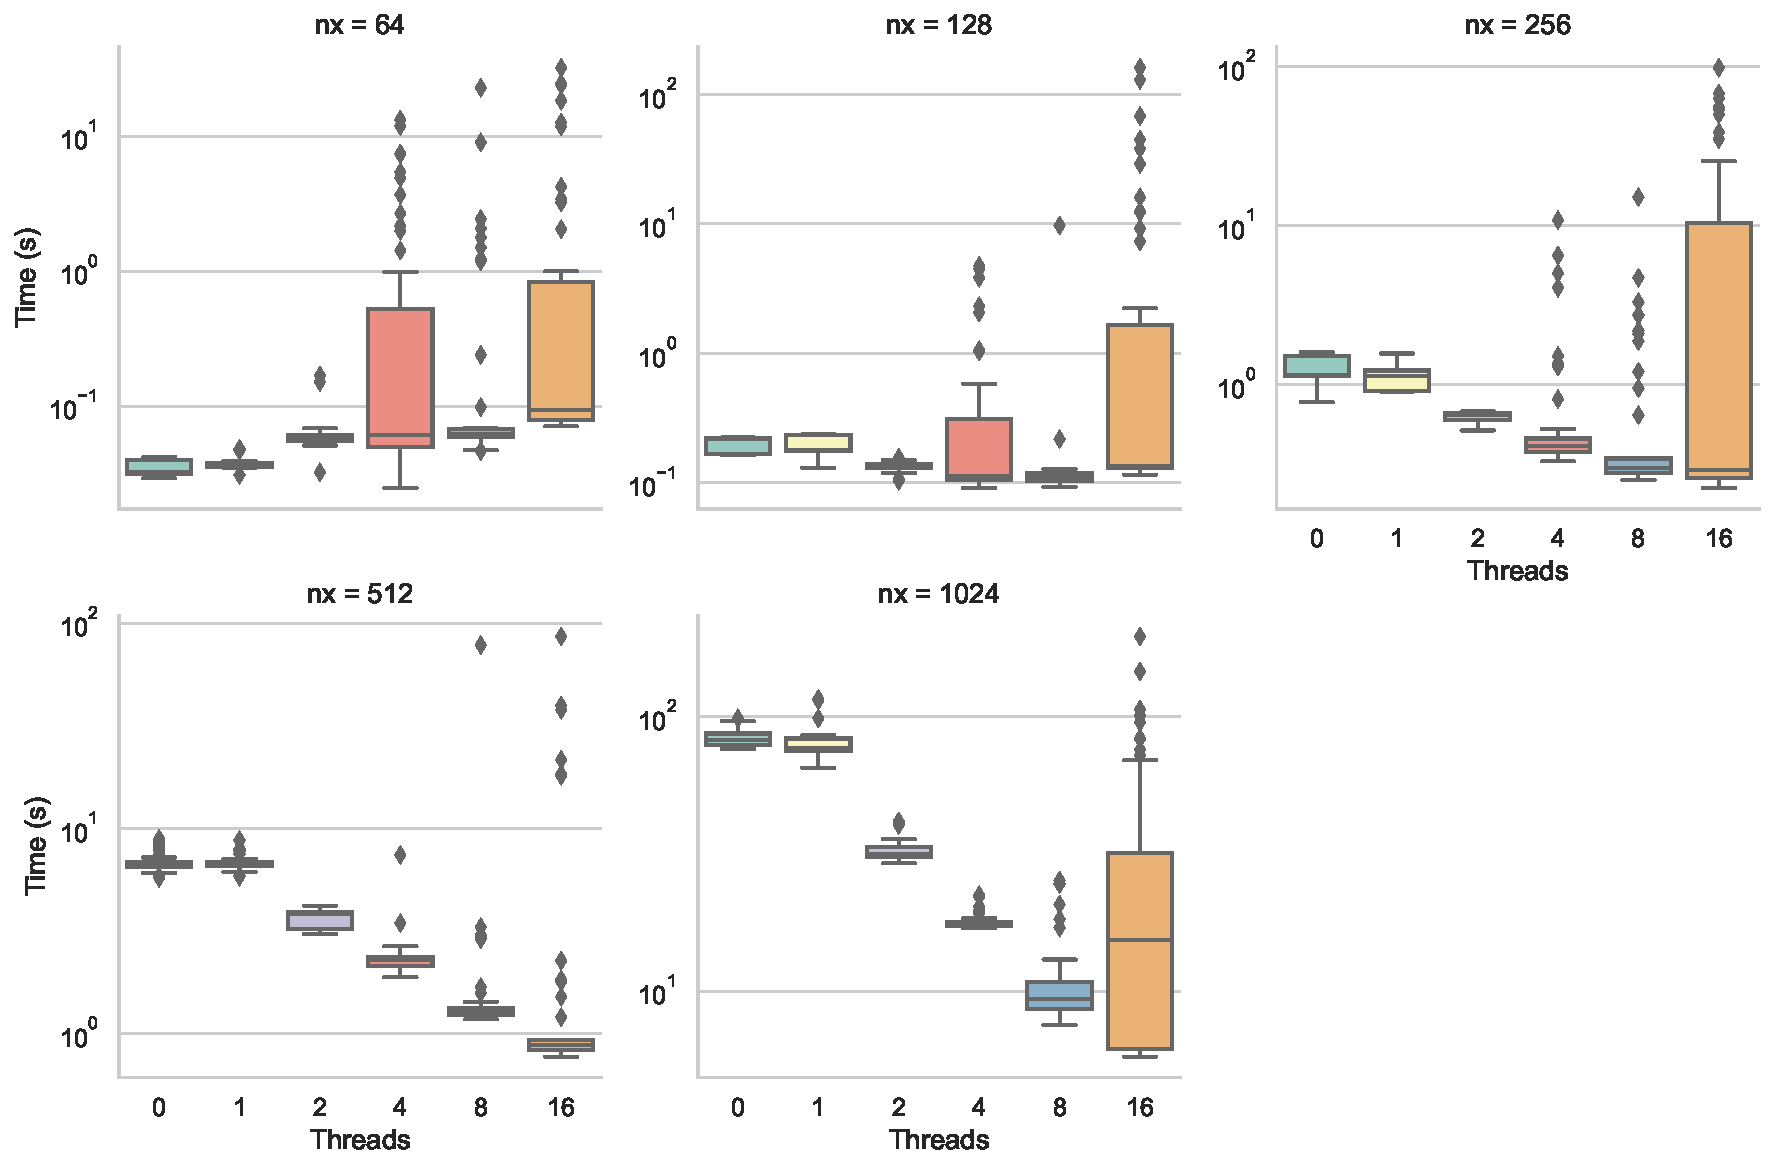
\includegraphics[width=\textwidth]{../mini_app/data_var.pdf}
    \caption{Time taken for the serial and parallel versions of the code; zero threads indicates serial version.}
    \label{im:times}
\end{figure}
Since the run times are so variable, I decided to use the median of the run
times
to determine the run time for the strong and weak scaling experiments. We can
see that specially when using 16 threads, the variability is very high and there
is a large number of outliers. This puts into question how relliable is
benchmarking on the Euler cluster. There is also the interesting case of 4
threads on a $64\times64$ grid which seems to have very high run times compared
to the other cases. I wonder if this has something to do with hardware.

The results of the strong scaling are shown in Fig. \ref{im:strong_scaling}
\begin{figure}[!h]
    \centering
    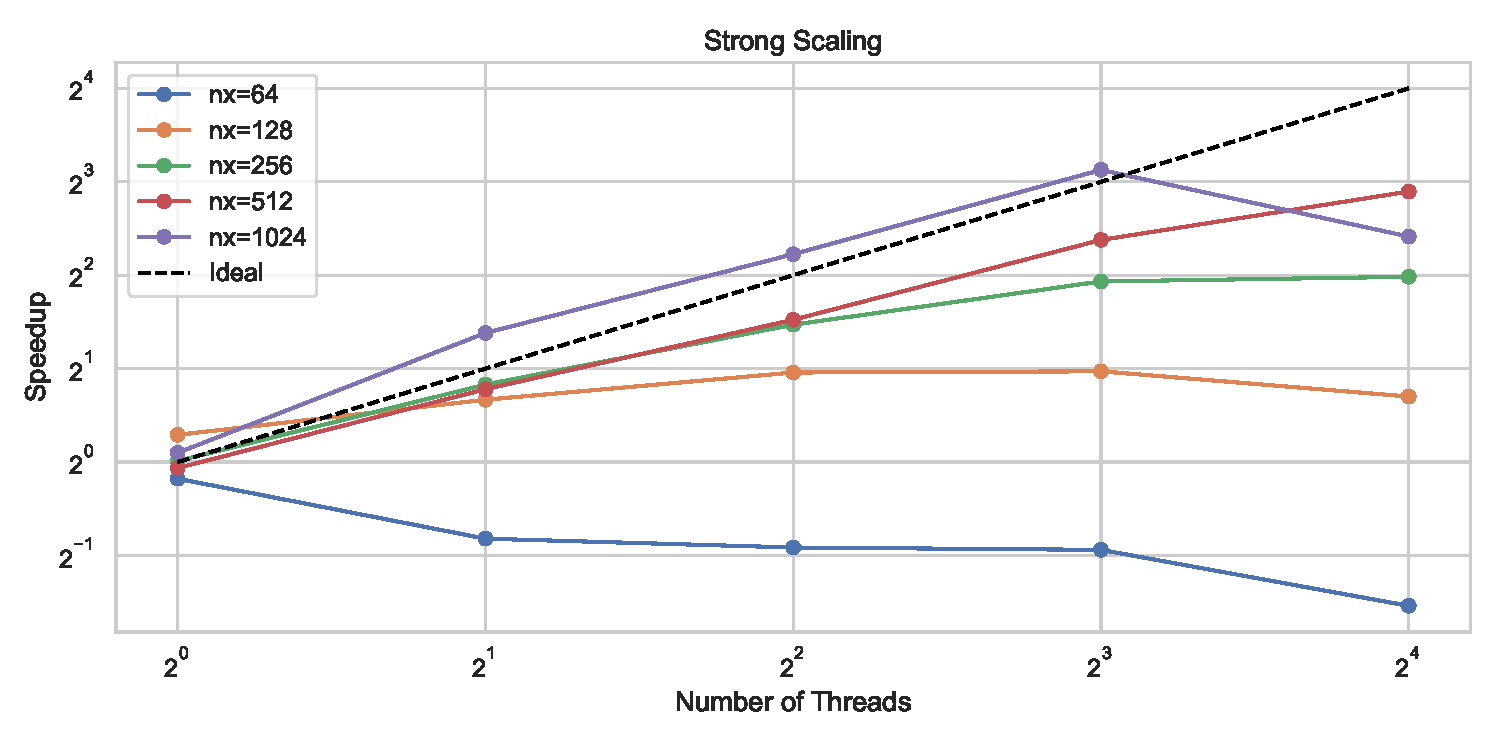
\includegraphics[width=\textwidth]{../mini_app/strong_scaling_plot.pdf}
    \caption{Strong scaling of the code.}
    \label{im:strong_scaling}
\end{figure}
The beyond optimal performance can be explained by the chosen representative of
the time in the serial and parallel versions. The plot shows that the parallel
implementation is doing a good job at scaling with the number of threads when
the grid size is at a certain level that is not too small.
At first, running it with a small grid size, the parallel version does not show
an improvement in performance. This can be explained with the overhead of
parallelizing the  code. But we can see that as the grid size increases, the
parallel version is able to take advantage of the multiple threads and the
performance improves.

\subsection*{Weak scaling}
For the weak scaling, I ran the code for the parallel verison 100 times for each
combination of threads and grid size. 
Following the previous analysis of run times, I again
used the median as representative. 
The results are shown in Fig. \ref{im:weak_scaling}.

\begin{figure}[!h]
    \centering
    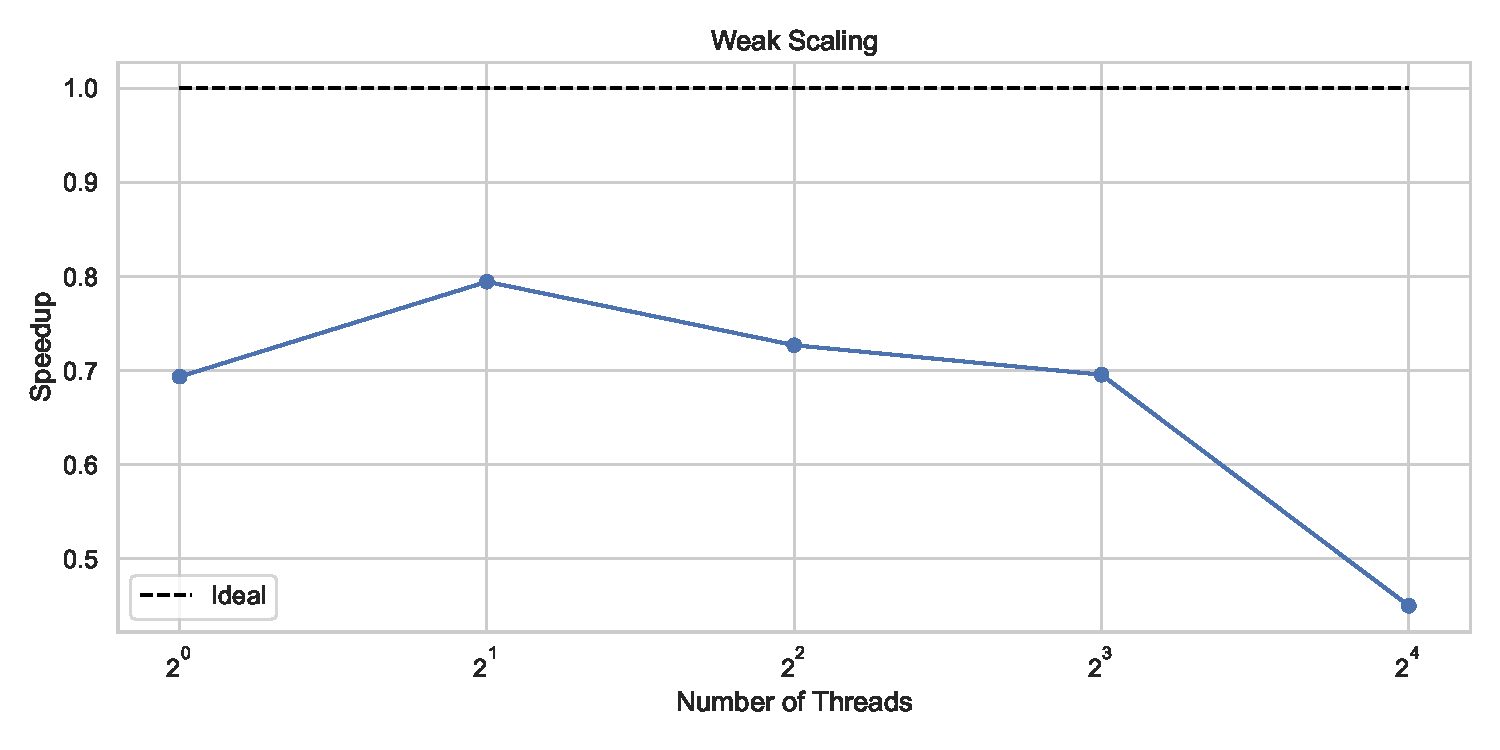
\includegraphics[width=\textwidth]{../mini_app/weak_scaling_plot.pdf}
    \caption{Weak scaling of the code.}
    \label{im:weak_scaling}
\end{figure}
The figure shows that the parallel version is able to scale well with the grid,
although not reaching the ideal performance, which is expected. The performance
is still good, reaching mostly around 0.7, except for the case of 16 threads. As
discussed before, this configuration seems to have a large variability in the
run times.

\end{document}
